% !TEX TS-program = XeLaTeX
% use the following command: 
% $ xelatex -shell-escape -output-driver="xdvipdfmx -z 0" article.tex
% this "-z 0" must be used to suppress compression in XMP Metadata packet 
% all document files must be coded in UTF-8
\documentclass{textolivre}
% for anonymous submission
%\documentclass[anonymous]{textolivre}
% to create HTML use 
%\documentclass{textolivre-html}
% remove all auxiliary files
% find . -name 'tl-article-template.*' ! -name '*.tex' ! -name '*.pdf' ! -name '*.bib' -type f -exec rm {} \;
% HTML compile using make4ht
% $ make4ht -c textolivre-html.cfg -u -x article "fn-in,svg"   # or use `mathjax' instead of `svg' to get LaTeX equation that will be handled by MathJax
% $ bibtex article
% clean and prettify HTML 
% $ tidy -o article-tidy.html --output-xhtml --break-before-br --wrap 0 article.html 2> errs.txt
% https://www.html-tidy.org/documentation/

% Metadata
\begin{filecontents*}[overwrite]{article.xmpdata}
    \Title{Dictionnaires contextuels: pour une approche ergonomique de la biotraduction}
    \Author{Wafa Bedjaoui \sep Bahia Zemni \sep Hayfa Almalki \sep Marwa Elsaadany}
    \Language{fr}
    \Keywords{Traduction contextuelle \sep Traduction collaborative \sep Traduction arabe-français \sep Dictionnaires contextuels \sep Corpus parallèles}
    \Journaltitle{Texto Livre}
    \Journalnumber{1983-3652}
    \Volume{14}
    \Issue{1}
    \Firstpage{1}
    \Lastpage{15}
    \Doi{10.35699/1983-3652.2021.25577}

    \setRGBcolorprofile{sRGB_IEC61966-2-1_black_scaled.icc}
            {sRGB_IEC61966-2-1_black_scaled}
            {sRGB IEC61966 v2.1 with black scaling}
            {http://www.color.org}
\end{filecontents*}

% PDF/A
% - install package icc-profiles
% - it is necessary to convert all image files to PDF/A
%   use ghostscript as shown below:
%   PDF images:
%   $ gs -dPDFA -dBATCH -dNOPAUSE -sColorConversionStrategy=UseDeviceIndependentColor -dCompatibilityLevel=1.4 -sDEVICE=pdfwrite -sProcessColorModel=DeviceCMYK -dPDFACompatibilityPolicy=2 -sOutputFile=figure-a.pdf figure.pdf
%   Other images:
%   $ convert figure.png figure.eps
%   $ gs -dPDFA -dBATCH -dNOPAUSE -sColorConversionStrategy=UseDeviceIndependentColor -dCompatibilityLevel=1.4 -sDEVICE=pdfwrite -sProcessColorModel=DeviceCMYK -dPDFACompatibilityPolicy=2 -dEPSCrop -sOutputFile=figure.pdf figure.eps

\journalname{Texto Livre: Linguagem e Tecnologia}
\thevolume{14}
\thenumber{1}
\theyear{2021}
\receiveddate{\DTMdisplaydate{2020}{05}{15}{-1}} % YYYY MM DD
\accepteddate{\DTMdisplaydate{2020}{08}{13}{-1}}
\publisheddate{\DTMdisplaydate{2020}{09}{29}{-1}}
%% Corresponding author
\corrauthor{Wafa Bedjaoui}
%% DOI
\articledoi{10.35699/1983-3652.2021.25577}
% list of available sesscions in the journal: articles, dossier, reports, essays, reviews, interviews, editorial
\articlesessionname{Tradução e Tecnologia}
%% Abbreviated author list for the running footer
\runningauthor{Bedjaoui et al.}
\editorname{Leonardo Araújo}

\title{Dictionnaires contextuels: pour une approche ergonomique de la biotraduction}
\othertitle{Dicionários contextuais: para uma abordagem ergonômica da biotranslação}
\othertitle{Contextual dictionaries: for an ergonomic approach of biotranslation}

\author[1]{Wafa Bedjaoui \orcid{0000-0002-0660-8418} \thanks{Email: \url{wfbedjaoui@pnu.edu.sa}}}
\author[1]{Bahia Zemni \orcid{orcid.org/0000-0002-6238-7509} \thanks{Email: \url{baalzemni@pnu.edu.sa}}}
\author[1]{Hayfa Almalki \thanks{Email: \url{haalmalki@outlook.sa}}}
\author[1]{Marwa Elsaadany \orcid{0000-0002-6867-4250} \thanks{Email: \url{maabdelFatah@pnu.edu.sa}}}

\affil[1]{Princess Nourah bint Abdulrahman University, Riyadh, Arabie Saoudite.}

%\usepackage[backend=biber,style=abnt, ittitles]{biblatex}
%\DeclareLanguageMapping{brazil}{brazil-apa}
\addbibresource{article.bib}     
% use biber instead of bibtex
% $ biber tl-article-template
% $ pdflatex tl-article-template.tex

% set language of the article
\setdefaultlanguage{french}
%\newfontfamily\frenchfont[Script=French]{SourceSansPro}
\setotherlanguages{english,portuguese}
\setotherlanguage{arabic}
\newfontfamily\arabicfont[Script=Arabic]{Amiri} 
\newfontfamily\arabicfontsf[Script=Arabic]{Amiri}
\newfontfamily\arabicfonttt[Script=Arabic]{Amiri}

\begin{document}
\maketitle

\begin{polyabstract}
\begin{abstract}
Le but de cet article est de mettre en évidence les fonctionnalités des corpus en ligne à l'instar des concordanciers, 
notamment le dictionnaire contextuel Reverso Context. À travers cette étude exploratoire, nous cherchons à connaître les limites 
de ce dictionnaire contextuel en ligne de l'arabe vers le français en analysant la traduction dans le contexte des adages arabes 
traduits en français. Il s'agit aussi de mettre en exergue la notion de collaboration virtuelle proposée dans le cadre du 
dictionnaire collaboratif de Reverso Context. L'étude a également permis de décrire les prestations et les fonctionnalités 
proposées en ligne de ce dictionnaire ainsi que ses limites. A travers l'expérimentation de la traduction des adages et des 
proverbes de l'arabe vers le français, nous avons pu déduire que le dictionnaire contextuel Reverso Context présente des limites 
de traduction en ce qui concerne les combinaisons arabe-français. Ces limites sont d’ordre lexical, sémantique, phrastique et 
rhétorique. Sans oublier que ses bases de données lexicales et terminologiques sont faiblement alimentées en langue arabe.

\keywords{Traduction contextuelle \sep Traduction collaborative \sep Traduction arabe-français \sep Dictionnaires contextuels \sep Corpus parallèles}
\end{abstract}

\begin{english}
\begin{abstract}
The purpose of this article is to highlight the functionalities of online corpora such as concordancers, 
in particular the Reverso Context Dictionary. Through this exploratory study, we seek to know the limits 
of this online contextual dictionary from Arabic to French by analyzing the translation in the context of 
Arabic adages translated into French. It also aims to highlight the notion of virtual collaboration proposed 
within the framework of the Reverso Context collaborative dictionary. The study also made it possible to 
describe the services and functionalities offered online by this dictionary as well as its limitations. 
Through the experimentation of the translation of adages and proverbs from Arabic into French, we were able 
to deduce that the Reverso Context contextual dictionary has translation limits regarding Arabic-French 
combinations. These limits are lexical, semantic, phrasal and rhetorical.

\keywords{Contextual translation \sep Collaborative translation \sep Arabic-French translation \sep Contextual dictionaries \sep Parallel corpora}
\end{abstract}
\end{english}

\begin{portuguese}
\begin{abstract}
O objetivo deste artigo é destacar as funcionalidades dos corpora online como concordanciadores, 
em particular o dicionário contextual Reverso Context. Por meio deste estudo exploratório, buscamos 
conhecer os limites desse dicionário contextual online do árabe para o francês, analisando a tradução 
no contexto dos ditados árabes traduzidos para o francês. Trata-se também de destacar a noção de 
colaboração virtual proposta no âmbito do dicionário colaborativo Reverso Context. O estudo também 
possibilitou descrever os serviços e funções oferecidos online por esse dicionário, bem como suas 
limitações. Por meio da experimentação com a tradução de ditados e provérbios do árabe para o francês, 
pudemos concluir que o dicionário Reverso Context tem limitações de tradução no que diz respeito às 
combinações árabe-francês. Esses limites são lexicais, semânticos, fraseados e retóricos. Observamos, 
ainda, que suas bases de dados lexicais e terminológicas são mal fornecidas em árabe.

\keywords{Tradução contextual \sep Tradução colaborativa \sep Tradução \'{a}rabe-franc\^{e}s \sep Dicionários contextuais \sep Corpus paralelos.}
\end{abstract}
\end{portuguese}
\end{polyabstract}


\section{Introduction}\label{sec-intro}
Les traducteurs du XXI siècle font face au défi de l’information instantanée en flux et des méga-bases de données. Pour gagner plus de temps, on a recours à des dictionnaires en ligne qui, en un clic, donnent d’innombrables définitions, voire d’innombrables traductions d’un seul et même mot. Le traitement des langues naturelles par la machine se développe depuis plus de 60 ans. La traduction proposée dans le cadre de la traduction en ligne\footnote{
Cette expression désigne tous les types de traductions à l’aide de la machine (traduction automatique, contextuelle, concordanciers, corpus parallèles, statistique, traduction neuronale).
} 
s’est considérablement développée depuis. Des dictionnaires monolingues, bilingues voire trilingues et quadrilingues proposent des milliers de choix aux traducteurs. Leur nomenclature a été diamétralement révolutionnée ainsi que les méthodes de leur appréhension. Il ne s’agit plus de chercher les vocables par ordre alphabétique. Et les définitions ne sont plus offertes hors contexte. Une autre caractéristique à retenir, c’est que les dictionnaires en ligne ne sont plus l’apanage des érudits, puisque les praticiens de la langue et de la traduction apportent leurs contributions grâce aux espaces collaboratifs consacrés à d’autres suggestions que celles proposées par ces dictionnaires en ligne.

De nombreux outils de traduction d’aide à la traduction se concurrencent sur le marché: Systran, Bing translator, U dictionnary, Linguee. Cependant, en dépit de la qualité de la traduction offerte, le U dictionnary et Systran n’offrent pas les combinaisons arabe-français et français-arabe. C’est pourquoi nous avons opté pour Reverso Context puisqu’il répond aux exigences de notre recherche relatives à la traduction contextualisée et offre des traductions assez satisfaisantes aux traducteurs. C’est ce qui a été confirmé par une enquête  que nous avons menée auprès de quelques traducteurs répartis dans deux régions différentes : la Maghreb et le Moyen Orient\footnote{
Nous allons présenter quelques résultats dans les pages suivantes.
}.

La réflexion du présent travail de recherche a été nourrie par une première remarque selon laquelle les traductions suggérées par les dictionnaires contextuels à l’instar de Reverso Context, en tant que concordancier\footnote{
Les concordanciers sont des outils de recherche et d’aide à la traduction dans lesquels sont alignés des phrases et leurs traductions à partir de corpus parallèles. 
}, manquent de précision et sont erronées notamment quand il s’agit de traduire les adages et les proverbes arabes vers le français. Le choix de ces derniers s’explique par leur nature brève et métaphorique pour véhiculer la sagesse de toute une nation. Nous ambitionnons appréhender leur traduction à travers l’alignement du concordancier.

Nous y interrogerons également l’environnement numérique et l’ergonomie de la traduction humaine ou biotraduction\footnote{
Rudy Loock propose le terme de biotraduction pour désigner la traduction humaine par rapport à la traduction automatique.
} \cite{loock2019} en contexte numérique et digitalisé. C’est aussi poser la question de l’apport et des limites du dictionnaire contextuel Reverso Context ainsi que le rôle des traducteurs collaborateurs à ce service de traduction en termes de post-édition \cite{deneufbourg2019}. Nous partons de l’idée selon laquelle les dictionnaires contextuels sont des outils d’aide à la traduction pour permettre au traducteur de mener son travail dans des conditions optimales.

Il ne s’agit pas, dans cet article, de parler des internautes qui ont besoin d’une traduction rapide, mais des professionnels de la traduction dans leur usage des dictionnaires contextuels. Il ne s’agit pas non plus de vérifier si ces logiciels sont performants ou pas par rapport à l’humain. Là n’est pas notre objectif. Ainsi, nous nous proposons d’interroger le processus du traitement de l’entrée source et sa restitution à l’entrée cible. Par « entrée »\footnote{
Ce concept nous l’avons emprunté à la lexicographie.
} nous désignons le mot ou l’expression qui fait l’objet de la traduction au niveau du concordancier de Reverso Context. 

Cette recherche est menée dans une perspective interventionniste dans l’objectif d’alimenter les ressources du traducteur des combinaisons arabe-français-arabe, d’autant plus que les dictionnaires contextuels sont principalement des dictionnaires collaboratifs. Le principe est de proposer des traductions à celles déjà existantes afin d’améliorer leur qualité ou de proposer des traductions à des expressions qui ne figuraient pas dans les bases de données du dictionnaire. Cette étude s’inscrit ainsi dans le paradigme traductologique de l’approche de l’étude de la traduction par les corpus. Elle soulève les questions épistémologiques relatives aux outils TAO à l’instar de Reverso Context.


\section{Tour d’horizon des travaux sur la traduction en ligne}\label{sec-tour}
Malgré la capacité des machines d’effectuer avec succès des calculs mathématiques complexes, les traductions produites électroniquement sont toujours pleines d’erreurs \cite[p. 1]{yen2013}. Quand \cite{yen2013} parle de calcules mathématiques, il fait référence à la traduction Automatique Statistique (la traduction neuronale n’étant pas encore utilisée par les moteurs de TA en 2013). Reverso Context fait partie des concordanciers (TAO) ; et donc ses erreurs sont le résultat d’un alignement machinal (non corrigé) des corpus parallèles, et non pas de la traduction automatique proprement dite. Selon \textcite[p. 3]{loock2016}:

\begin{quote}
L’utilisation de ce type de corpus (parallèles) comme outil d’aide à la traduction est très répandue (et donc consensuelle); on les trouve sous la forme de mémoires de traduction, de   corpus   en   ligne   disponibles   sur   des   sites   internet   comme   les   très   en   vogue \url{www.linguee.com} ou  \url{www.reverso.net}.
\end{quote}

Avec l’avènement de la traduction automatique neuronale (TAN) en 2015, la qualité des traductions produites sont nettement meilleures. Il suffit de tester DeepL Translator. Relativement nouvelle en tant que paradigme, la traduction neuronale n’est pas l’objet de notre propos dans cette contribution surtout que la langue arabe ne figure pas parmi les langues faisant partie du répertoire des combinaisons des langues proposées. Sans oublier que la traduction automatique qu’elle soit à base de règle, de statistiques ou neuronale ne connait pas dans le monde arabe les mêmes développements qu’en Europe qui est le lieu de nouvelles configurations économiques relatives au métier du traducteur. D’après un rapport des Nations Unies:

\begin{quote}
Si la langue arabe tarde à s’imposer sur la toile, c’est aussi en raison du taux élévé d’illétrisme dans le monde arabe et d’un taux d’accès à internet encore faible. L’anglais est roi et la langue arabe, parlée par 4,5\% de la population mondiale, occupe moins de 1\% sur la toile \cite{euronews2016}.
\end{quote}

Selon \cite{loock2019}, en 2018, la proportion d’entreprises de services linguistiques européennes déclarant avoir recours à la TA a dépassé pour la première fois les 50\% conformément à l’étude publiée sur les langues européennes en 2018\footnote{
European Language Industry Survey: \url{https://ec.europa.eu/info/sites/info/files/2017_language_industry_survey_report_en.pdf}
}. L’utilisation de la TA au sein des logiciels de traduction assistée par ordinateur (par exemple SDL Trados Studio, memoQ), sous la forme de fonctionnalité intégrée ou de plug-in\footnote{
Plug in veut dire en informatique les nouvelles fonctionnalités ajoutées à celles de départ.
}, se généralise. 

Une première observation des dictionnaires en ligne nous permet de constater la forte présence de la langue anglaise \cite{gaudiaut2019}, en tant que première langue mondiale de laquelle et vers laquelle on traduit. Quant à la langue arabe, elle est faiblement alimentée dans les différents sites et applications\footnote{
On parle d’application quand les programmes ou les logiciels proposent leurs services sur les smartphones. 
} de traductions à l’instar de Google translate et  de Reverso Context puisque nous rencontrons, en tant que traductrice professionnelle, beaucoup de difficultés quand il s’agit de traduire entre l’arabe et les langues indoeuropéennes (ambiguïté, construction phrastique erronée, erreurs de langue, etc.). Sans oublier la qualité médiocre de la traduction proposée de et vers l’arabe. 

Les travaux relatifs à la traduction contextualisée, aux dictionnaires contextuels et aux concordanciers dans le monde arabe n’ont pas fait l’objet de recherches scientifiques rigoureuses jusqu’à présent. Nous osons dire que les recherches dont il était question se rapportaient soit à la didactique de la traduction et aux avantages de l’insertion des nouvelles technologies dans l’enseig\-ne\-ment-apprentissage de cette discipline \cite{lahlou2016} et \cite{idir2019}, soit aux systèmes TAO en contexte égyptien \cite{husseini2014}\footnote{
Il existe certainement des travaux en langue arabe, mais qui se penchent principalement sur le traitement automatique de cette langue et non sur son étude d’un point de vue traductif et traductionnel. Il faut noter à cet égard que des thèses et des mémoires de masters en la matière se sont multipliés ces dernières années.
} ou algérien \cite{bedjaoui2016}. 

Même si les géants de la TAO arrivent quand même à fournir des traductions correctes à travers l’exploitation des corpus parallèles, il n’en demeure pas moins que la base architecturale de ces machines doit faire l’objet d’alimentation continue. Selon \cite{loock2017}, les corpus parallèles sont souvent segmentés et alignés au niveau de la phrase, ce qui n’est pas sans rappeler les mémoires de traduction que l’on trouve au sein des logiciels de traduction assistée par ordinateur (TAO) :  En ce sens, il s’agit pour les traducteurs d’exploiter les corpus comme source d’inspiration.

\section{Reverso Context:  État des lieux}\label{sec-reverso}
Depuis la création de Reverso en 1986 par le fondateur de Softissimo, spécialiste des logiciels et développement des langages, les supports en ligne à usage multilingue ont connu un grand essor: du correcteur grammatical au dictionnaire électronique en arrivant au dictionnaire contextuel Reverso Context.

Selon le développeur de Reverso \cite{hoffenberg2010}, la traduction a lieu dans 20 combinaisons de langues. Tout le monde peut s'inscrire et venir ajouter des définitions, des traductions mais également commenter les entrées des autres mem\-bres. À l’instar de Wikipedia, certains mem\-bres en fonction de la qualité et de la fréquence de leurs interventions corrigent et valident les entrées. 

Selon \textcite[p. 13]{ntakirutimana2007}, chaque unité lexicale dans une langue donnée y est reliée à ses équivalents sémantiques dans les autres langues. Le moteur syntaxique, quant à lui, sert à la reconnaissance des phrases. Il fonctionne comme un analyseur grammatical, décomposant chaque phrase de la langue de départ en ses structures syntaxiques. 

En tant que dictionnaire contextuel, Reverso Context, à l’instar des autres dictionnaires en ligne, a révolutionné les dictionnaires qui présentaient les équivalents abstraction faite de leur contexte. Il est ainsi possible de lire plusieurs propositions contextualisées à partir des corpus parallèles. Or, en dépit de cette révolution, nous avons constaté que des faiblesses demeurent à l’usage de ces outils puisque selon \textcite[p. 16]{yen2013}, la performance de Reverso était très irrégulière, troisième dans l’ensemble, deuxième pour les expressions idiomatiques et huitième en ce qui concerne les verbes à particules.

Avant d’entamer l’analyse des résultats obtenus, nous allons exposer quelques résultats d’une enquête que nous avons menée auprès de traducteurs amateurs et professionnels afin d’avoir une idée sur l’usage de Reverso Contexte en tant qu’outil de travail facilitateur de la pré-traduction, la traduction et  la post-traduction. L’enquête a été lancée en décembre 2019 et a duré un mois (janvier 2020) :  Le questionnaire a été établi à l’aide des formulaires de « google form » et a été distribué à travers le réseau social Facebook (sur les groupes des professionnels de la traduction) et à travers le courriel à des collègues. Nous avons recueilli 59 questionnaires\footnote{
Cette enquête ne vise pas la représentativité, mais a pour objectif de cerner les outils d’aide à la traduction les plus utilisés. Elle pourra être élargie ultérieurement.
}. Les deux zones géographiques principalement couvertes par l’enquête sont respectivement : le Maghreb et le Moyen-Orient comme le montre la \Cref{fig-01}.

\begin{figure}[htbp]
 \centering
 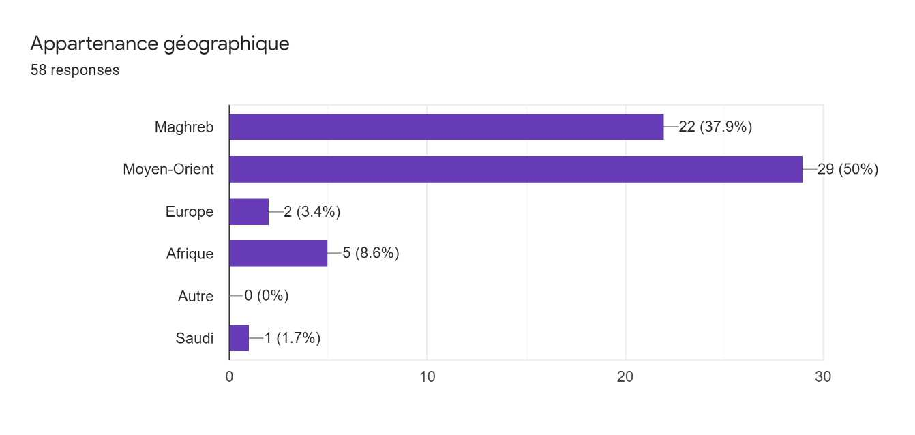
\includegraphics[width=0.85\textwidth]{figure01.pdf}
 \caption{Appartenance géographique.}
 \label{fig-01}
 \source{d'après les auteurs.}
\end{figure}

Les données obtenues mettent l’accent sur le positionnement géographique des enquêtés dont la langue maternelle est la langue arabe. Nous observons que 50\% répondants sont du Moyen-Orient et 37.9\% sont du Maghreb. Les pays du Moyen-Orient concernés sont l’Égypte, l’Arabie Saoudite et la Jordanie ; quant aux pays du Maghreb représentés dans l’enquête, il s’agit de l’Algérie, du Maroc et de la Tunisie.

La population ayant répondu aux questions est une population qui a un recours régulier et systématique à la traduction comme l’indique le \Cref{fig-02}.

\begin{figure}[htbp]
 \centering
 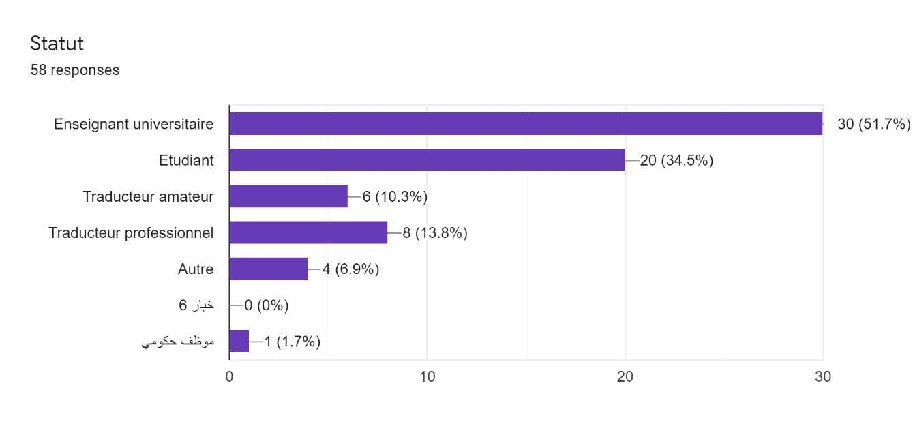
\includegraphics[width=0.85\textwidth]{figure02.pdf}
 \caption{Statut des enquêtés.}
 \label{fig-02}
 \source{d'après les auteurs.}
\end{figure}

A la question : Utilisez- vous des outils d’aide à la traduction? Nous avons obtenu le \Cref{fig-03}.

\begin{figure}[htbp]
 \centering
 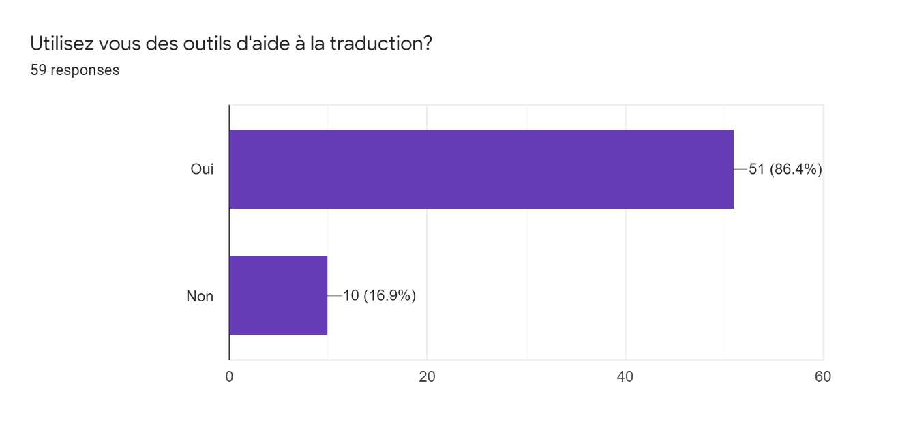
\includegraphics[width=0.75\textwidth]{figure03.pdf}
 \caption{Usage d’outils d’aide à la traduction.}
 \label{fig-03}
 \source{d'après les auteurs.}
\end{figure}

Cela étant, les traducteurs arabes de l’enquête sont à la page en matière de nouvelles technologies et leur usage dans le métier de la traduction avec un pourcentage de 86.4\% de oui à la question posée sur l’usage des outils d’aide à la traduction.

En réponse à une autre question relative à la qualité de la traduction en ligne , les traducteurs jugent que Reverso est le logiciel le plus fiable conformément au \Cref{fig-04}. 

\begin{figure}[htbp]
 \centering
 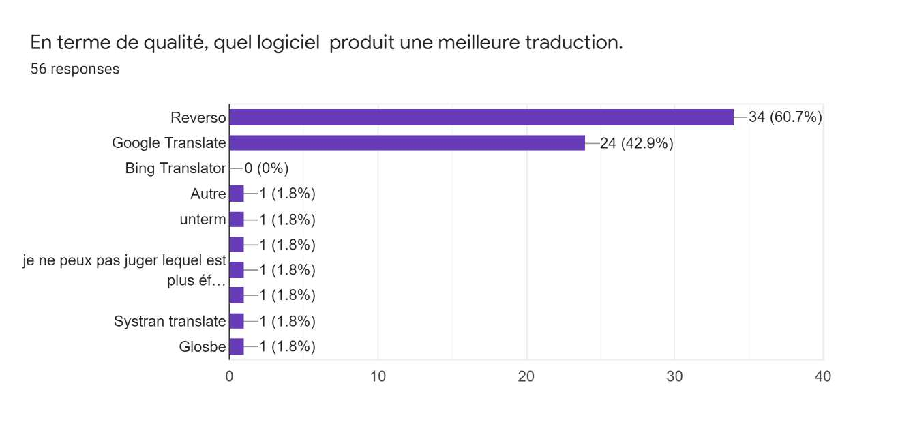
\includegraphics[width=0.85\textwidth]{figure04.pdf}
 \caption{Qualité des logiciels de traduction.}
 \label{fig-04}
 \source{d'après les auteurs.}
\end{figure}


Nous pouvons déduire que Reverso Context est l’outil d’aide à la traduction le plus utilisé par les traducteurs enquêtés avec un pourcentage de 60.7\% contre les autres outils qu’il s’agisse de traducteurs automatiques ou de concordanciers. 


\subsection{Services et fonctionnalités de Reverso Context}\label{sec-services}
En tant que base de connaissances collaboratives, le Reverso Context effectue des extractions de relations sémantiques qui lui permettent de donner des traductions dont le sens est généralement rendu. Cette opération d’extraction est facilitée par les corpus parallèles. En cas d’absence de propositions faites par le concordanciers, la traduction machinale intervient comme seule suggestion à la traduction du mot ou de l’expression recherchée.

Pour donner plus de précisions à nos propos, nous présentons les résultats d’une expérience menée dans le cadre de cette recherche pour vérifier l’efficacité de l’esprit collaboratif des dictionnaires contextuels à l’instar de Reverso Context. Nous avons demandé la traduction vers le français de l’expression «\textlang{arabic}{ أبناء الضاد }».
Le Reverso Context n’ayant pas trouvé l’alignement de cette expression dans les bases des corpus parallèles, nous a redirigé vers la traduction automatique du dictionnaire 
Reverso\footnote{
Reverso a plusieurs fonctionnalités : dictionnaire, correcteur grammatical, traducteur automatique, concordancier, localisateur.
}. Nous avons obtenu le résultat suivant conformément à la \Cref{fig-05}. 

\begin{figure}[htbp]
 \centering
 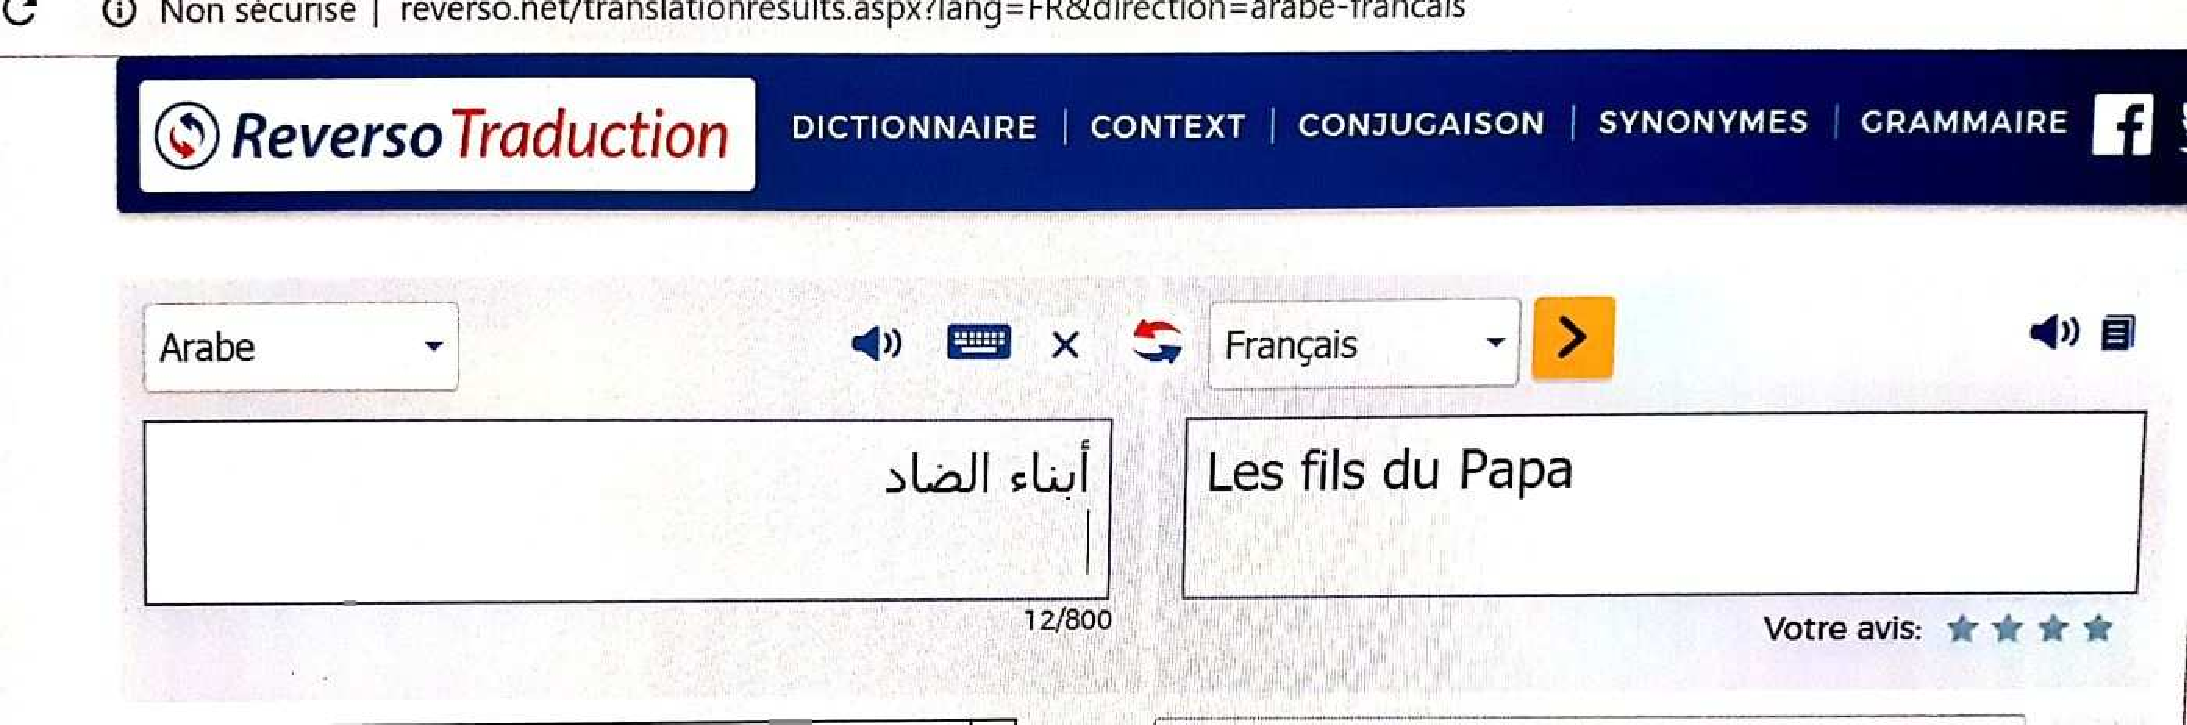
\includegraphics[width=0.75\textwidth]{figure05.pdf}
 \caption{Essai de traduction.}
 \label{fig-05}
 \source{d'après les auteurs.}
\end{figure}

Le moteur de traduction automatique de Reverso a proposé la traduction de la machine, qui est fausse, sans donner aucune autre suggestion des corpus parallèles ; ce qui nous amène à déduire que cette expression ne figure point dans les bases de données du dictionnaire.
\textlang{arabic}{ أبناء الضاد }
est une périphrase désignant les Arabes en tant que nation distinguée par une langue dont l’alphabet comprend une lettre (Alif, première lettre arabe, mentionnée après fils) qui n’existe dans aucune autre langue. L’option utilisée, à savoir la proposition de la traduction, ne change pas les résultats du concordancier, mais plutôt ceux de la traduction automatique proposés dans la première fenêtre de Reverso Context.

Dans la rubrique “Dictionnaire collaboratif”, nous avons soumis notre proposition de traduction de cette périphrase qui veut dire “Les Arabes” comme le montre la \Cref{fig-06}.

\begin{figure}[htbp]
 \centering
 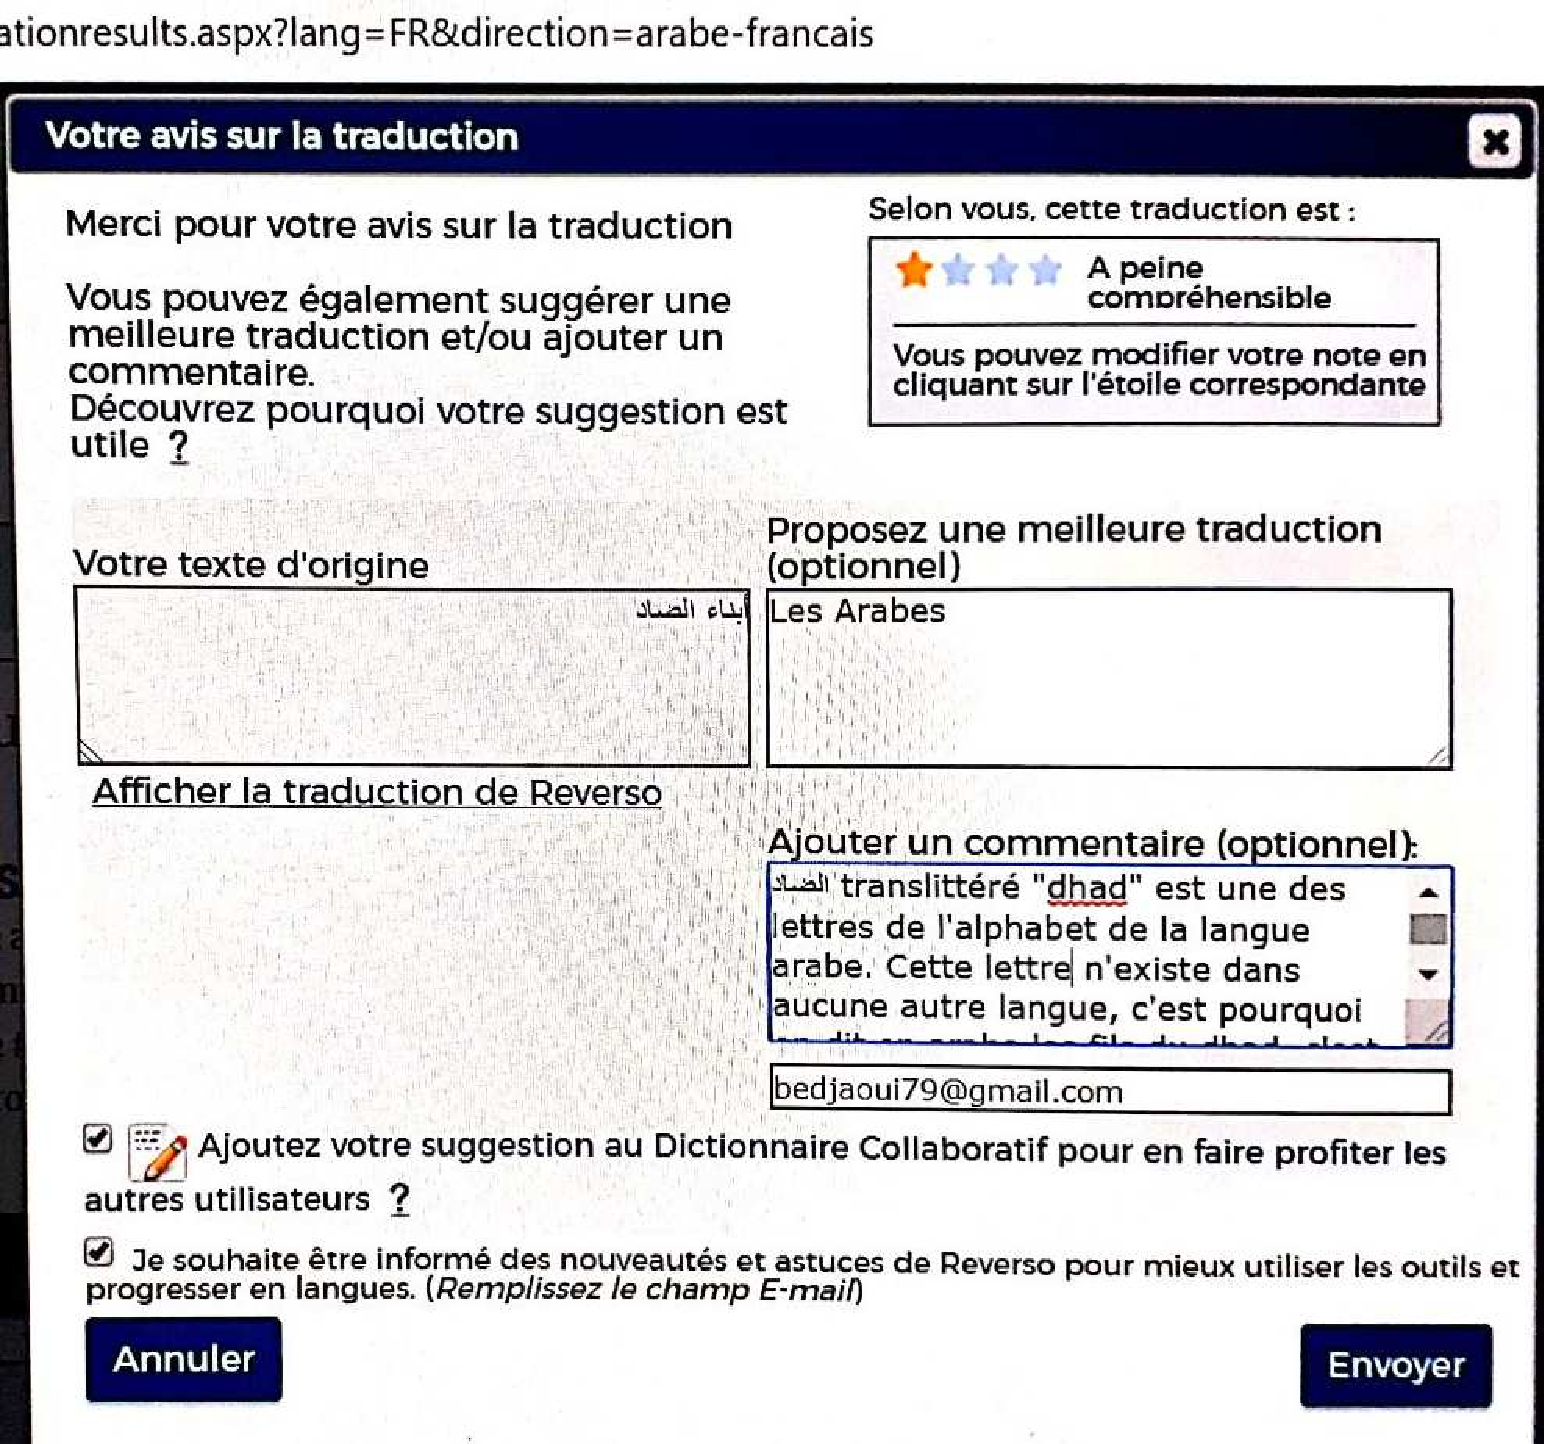
\includegraphics[width=0.75\textwidth]{figure06.pdf}
 \caption{Collaboration virtuelle.}
 \label{fig-06}
 \source{d'après les auteurs.}
\end{figure}

Après avoir ajouté la proposition et justifié la traduction, nous avons validé l’envoi pour qu’elle soit mise en ligne aux utilisateurs de la plateforme, mais avant la validation définitive, le logiciel nous a accompagné pour s’assurer de l’orthographe, de la catégorie grammaticale et d’autres points relatifs à la qualité de la langue vers laquelle on a traduit comme indiqué dans la \Cref{fig-07}. 

\begin{figure}[htbp]
 \centering
 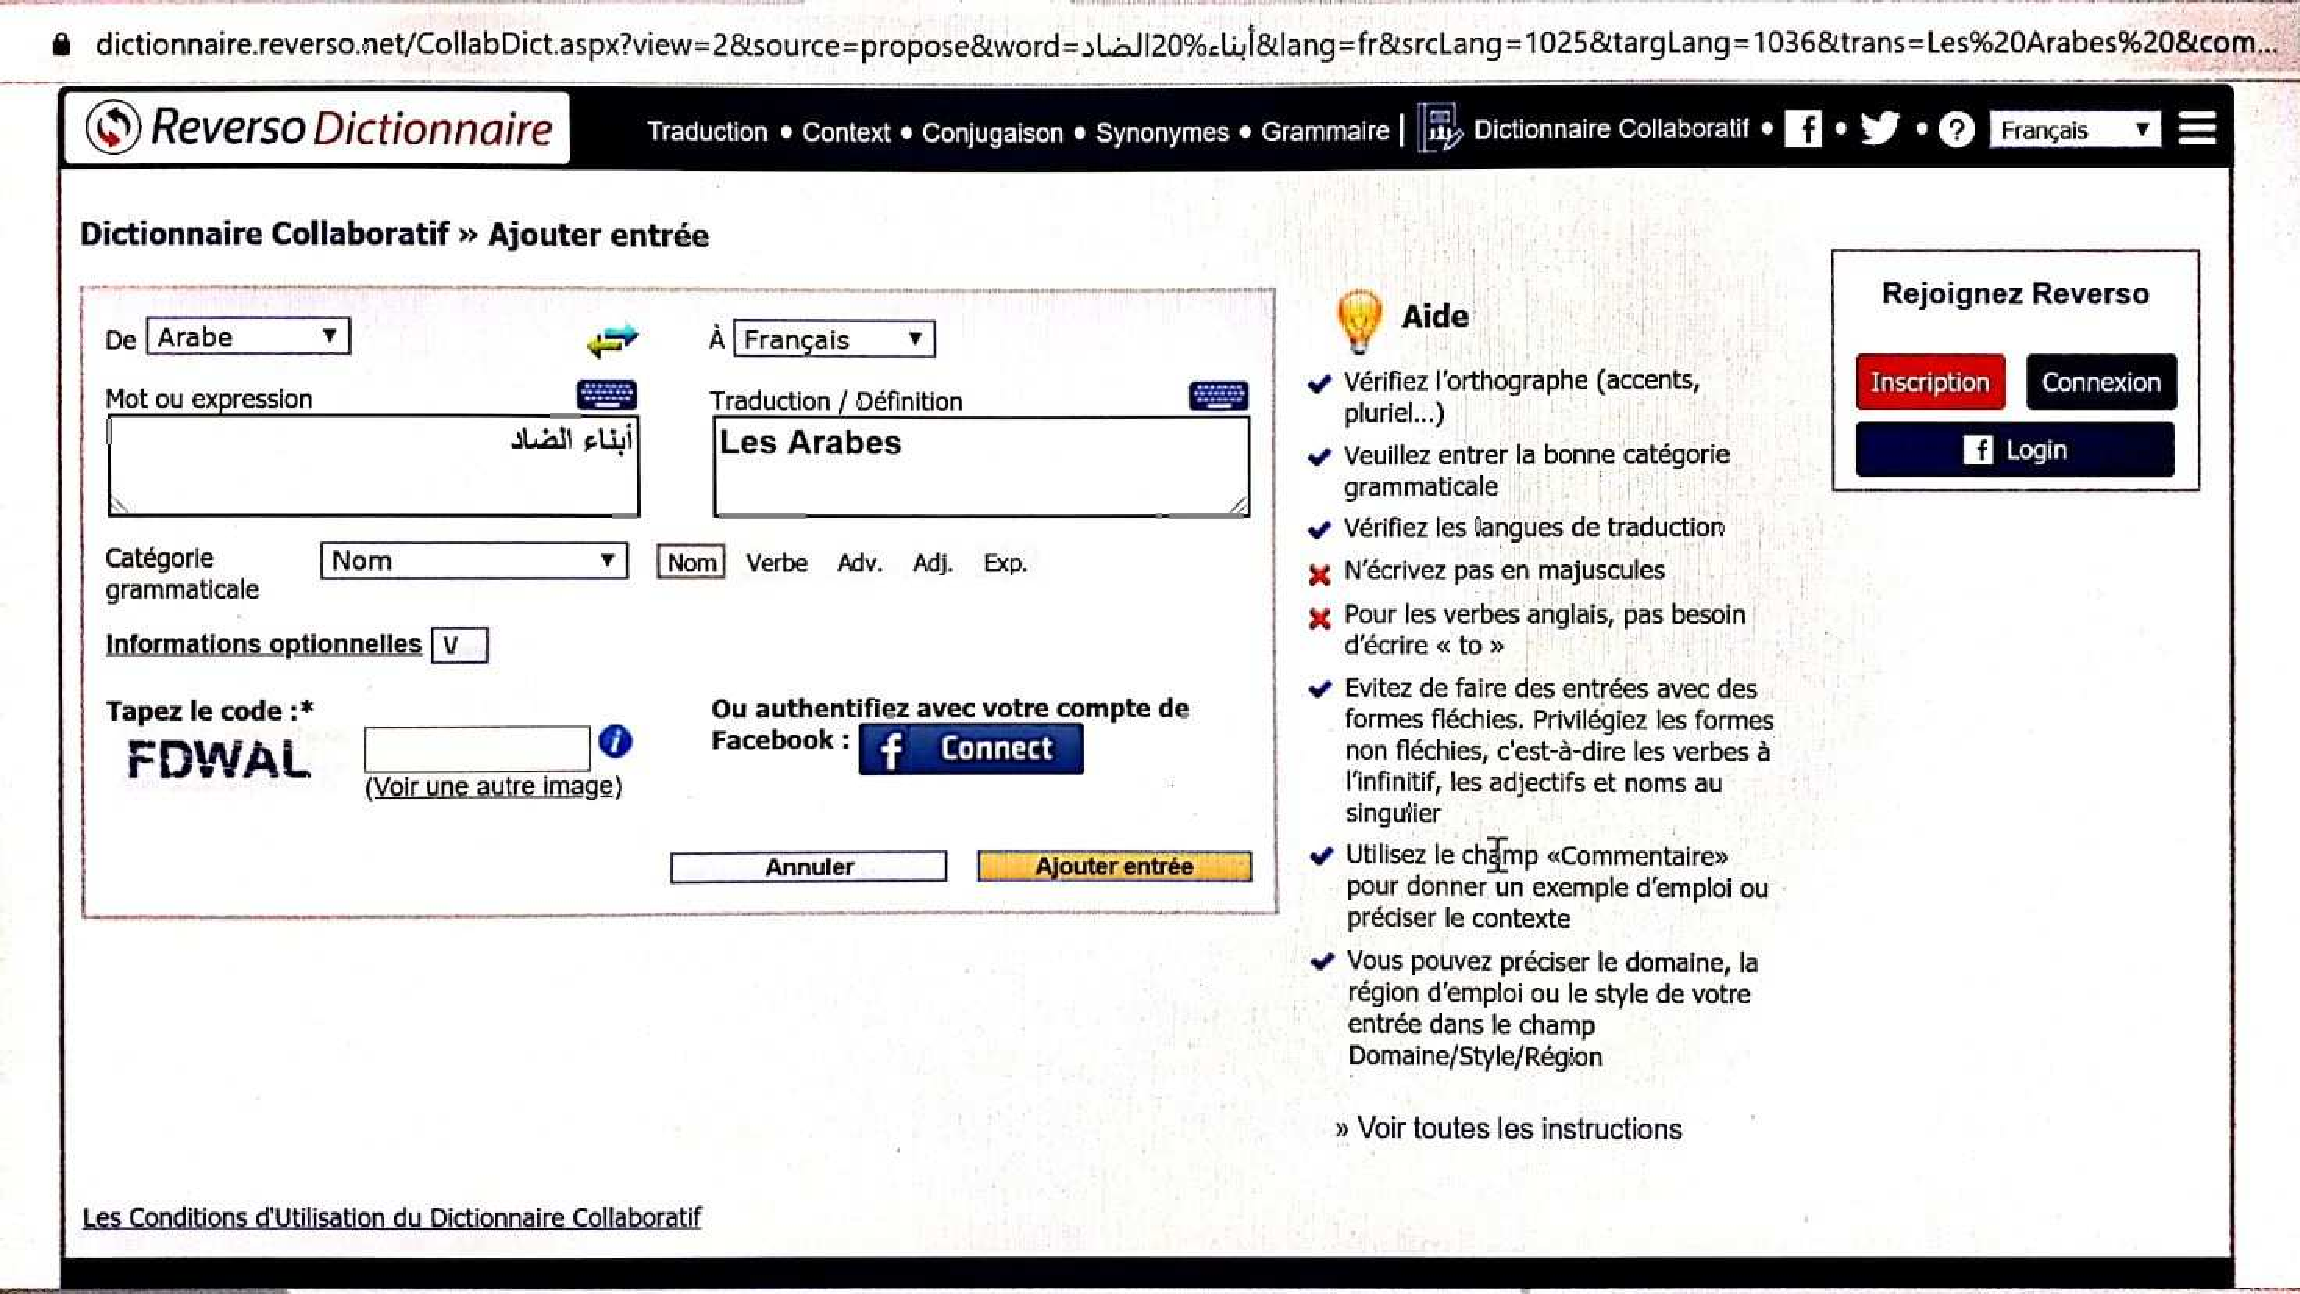
\includegraphics[width=0.75\textwidth]{figure07.pdf}
 \caption{Vérification de la proposition de traduction.}
 \label{fig-07}
 \source{d'après les auteurs.}
\end{figure}

Après quelques jours nous avons vérifié si le logiciel a accepté la proposition, il s’est avéré que oui comme le montre la \Cref{fig-08}. 

\begin{figure}[htbp]
 \centering
 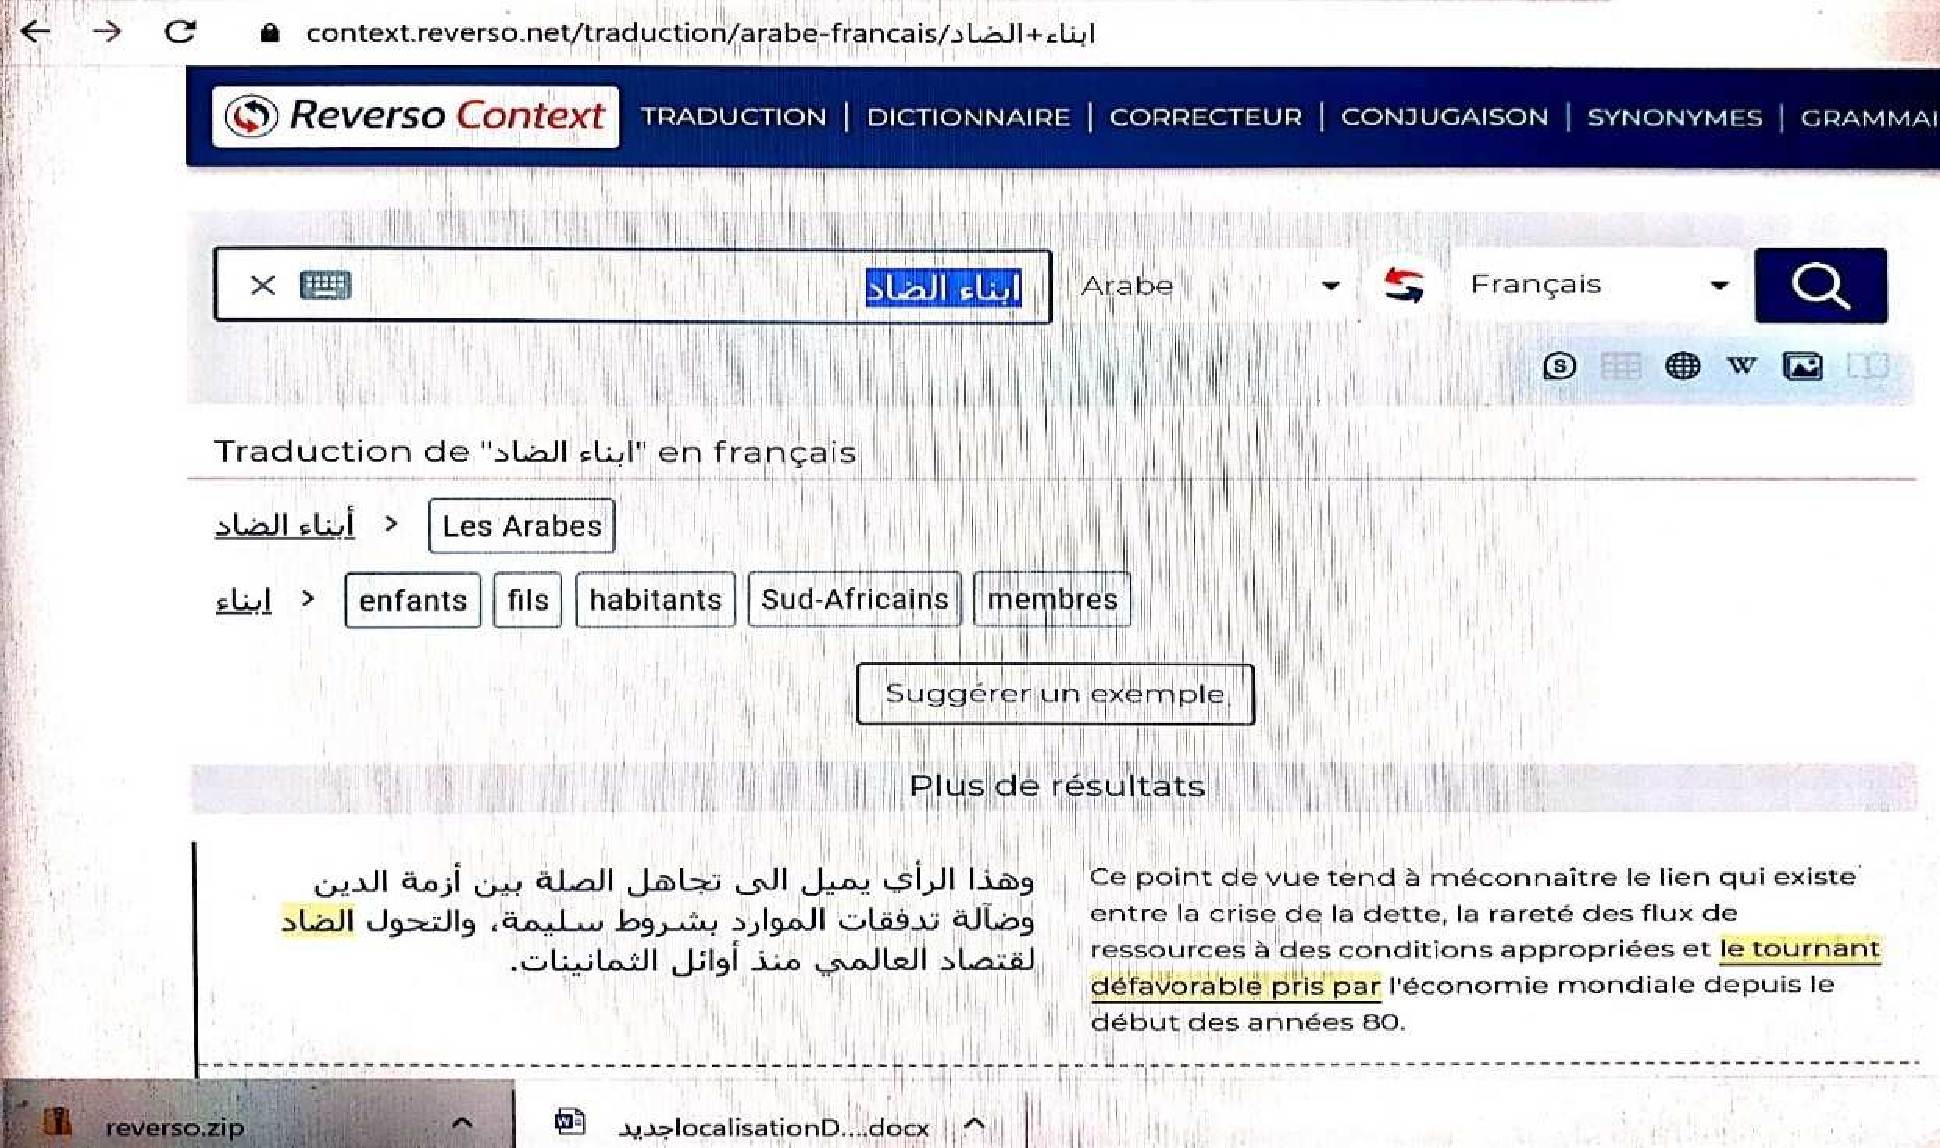
\includegraphics[width=0.75\textwidth]{figure08.pdf}
 \caption{Validation de la proposition.}
 \label{fig-08}
 \source{d'après les auteurs.}
\end{figure}

Force est de noter que cette proposition n’a pas été validée directement :  Reverso Context comprend une équipe de linguistes spécialistes qui vérifient le bien-fondé des suggestions pour pouvoir les adopter en tant que traduction fiable.

D’autres textes de typologies différentes ont été testés de la même façon pour vérifier la qualité de la traduction à savoir un extrait de l’essai philosophique « Le Mythe de Sisyphe » d’Albert Camus ainsi qu’un passage extrait du site français de l’ONU. Les textes produits dans la langue cible étaient lisible et ne posaient aucun problème d’ambiguïté en traduction du français vers l’arabe. 



\subsection{Limites des alignements des adages et des proverbes}\label{sec-limites}
L’une des caractéristiques des langues naturelles est leur caractère créatif, une seule idée peut être exprimée par d’innombrables énoncées. Nous représentons ce point par l’équation suivante : 

\begin{enumerate}
\item[] Une idée= des énoncés $\infty$
\item[] Soit l’idée suivante :  ‘une fille triste’ peut être formulée ainsi : 
\item Elle ne va pas bien
\item Elle se sent mal
\item Elle n’est pas dans son assiette
\item Elle est triste
\item Elle est mélancolique
\item Elle ressent du spleen
\item Elle souffre
\end{enumerate}

Et la liste est longue pour l’humain afin d’exprimer cette idée. Quant à la machine, elle est limitée au nombre des mots et des expressions injectés sur les bases de données des moteurs  de traduction que les développeurs alimentent à travers les corpus parallèles et/ou les algorithmes. Partant de ce constat, et devant l’impossibilité de combler toutes les situations de traduction en matière de choix traductifs alignés, nous allons appréhender les fonctionnalités des services fournies par le Reverso Context.

Afin de répondre à notre question de recherche et pour approfondir notre réflexion sur les limites des dictionnaires contextuels et les pistes à proposer pour remédier au manque en termes de traduction, nous avons sélectionné 20 adages et proverbes arabes que nous avons soumis à Reverso Context. Notre échantillon a été recueilli à partir de la rubrique “ adages et proverbes” du site Al maani\footnote{
\url{https://www.almaany.com/}
} qui met à la disposition des internautes arabes 600 adages et proverbes. Dans la sélection de notre corpus, nous avons tenu à ce que les expressions soient des expressions courantes dont les caractéristiques linguistiques relèvent de l’arabe moderne et standard\footnote{
L’arabe moderne appelé aussi standard est la langue enseignée à l’école et à l’université. C’est la langue de l’administration.
}. Nous avons ainsi exclu les dires du prophète Mohamed ainsi que les citations des penseurs arabes qui remontent à des dates lointaines dans l’histoire. Les traductions proposées ont fait l’objet d’une analyse contrastive sur les plans lexical, sémantique, et syntaxique.

Notre méthodologie d’analyse s’appuie sur une démarche qui relève des méthodes empirico-inductives, puisque les traductions produites par Reverso Context ont fait l’objet d’une observation et d’interprétation des erreurs.  Selon \textcite[p. 1]{chidi2005}, l’analyse de la typologie des fautes est utile pour l’avancement de la traduction. Avec l’avènement de la linguistique de corpus et du traitement automatique des données, il est possible aujourd’hui de recueillir bon nombre de productions réelles d’un traducteur donné pour les analyser afin de comprendre autant le traducteur lui-même que l’exercice de la traduction. 

Il est à noter que chaque langue a sa perception de la réalité et  que ses domaines de références sont partagés par une communauté donnée. Nous nous appuyons, pour cette section, sur les théories de la sémantique générative, ainsi que sur les théories de l'intelligence artificielle et de la traduction automatique, issues pour la plupart de la grammaire générative. Leur point commun est la recherche de la correspondance entre la structure de surface et le sens. Il s'agit de trouver les règles sémantiques qui s'associent à chaque représentation syntaxique et qui en conditionnent l'application \cite[p. 87]{Dancette1989}.

Nous avons retenu les traductions de la machine puisqu’elles étaient les seules proposées, et en cas d’absence de traduction de la machine nous avons sélectionné les traductions les plus récurrentes proposées par les corpus parallèles.

Une première observation des exemples recueillis nous a permis de constater que la fonctionnalité de la traduction automatique de Reverso Context est activée plus que les autres fonctionnalités à l’instar de l’alignement des corpus parallèles. Il suffit d’observer le Graphique 4 pour comprendre les sources des différentes propositions de traductions et d’équivalences.

\begin{figure}[htbp]
 \centering
 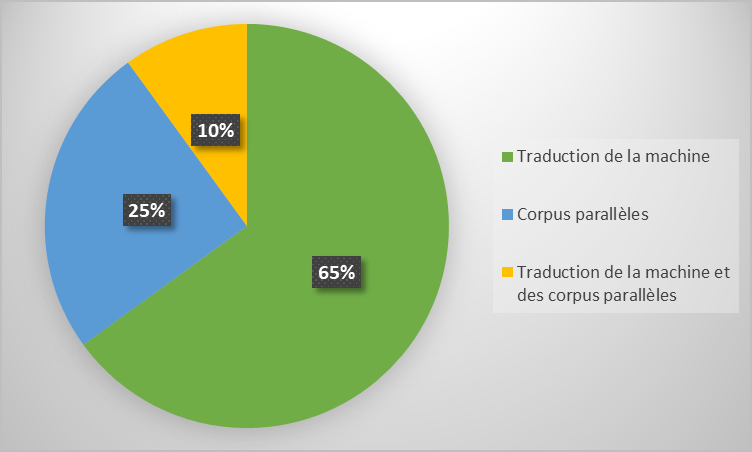
\includegraphics[width=0.75\textwidth]{figure09.pdf}
 \caption{Sources des traductions sur Reverso Context.}
 \label{fig-09}
 \source{d'après les auteurs.}
\end{figure}

65\% des traductions proposées sur Reverso Context sont celles de la machine, c’est-à-dire des traductions automatiques proprement dite. Les corpus parallèles ne constituent que 25\% des sources des propositions, ce qui demeure faible par rapport aux autres combinaisons de langues. La combinaison entre les deux fonctionnalités n’a enregistré que 10\%, ce qui indique que le traducteur professionnel n’a pas beaucoup de choix traductifs sur cette plateforme et doit soit post-éditer les propositions soit chercher dans d’autres ressources de corpus en ligne.

Le Tableau 1 ci-après constitue une grille d’analyse dans laquelle sont dégagés les remarques observées dans les traductions de Reverso Context.

%\setlength\LTleft{-1in}
%\setlength\LTright{-1in}
\begin{small}
\begin{longtable}{
    >{\raggedright\arraybackslash}p{0.1\textwidth}
    >{\raggedright\arraybackslash}p{0.34\textwidth}
    >{\raggedright\arraybackslash}p{0.04\textwidth}
    >{\raggedright\arraybackslash}p{0.4\textwidth}
    }    
\caption{Componentes e ferramentas.}
\label{tab01}
\\
\toprule
Finalidade & Material & Qtd & Fonte \\ \midrule
\multirow{3}{*}{Estrutura} & Chassi & 1 & ACM\footnote{\label{fnoteACM}Cuidado: condução elétrica na estrutura metálica do ACM.}, capa rígida de caderno \\ 
 & Roda dianteira & 1 & Roll-on labial ou de desodorante roll-on \\ 
  & Roda traseira & 2\footnote{\label{fnoteid}Precisam ser idênticos.} & Chinelo \\ 
\midrule
\multirow{10}{*}{\shortstack{Circuitos \\ Eletrônicos}} & Placa (fixar componentes) & 1 & placa ou pasta de plástico \\
 & Resistor $300\Omega$ (ou 1 de $220\Omega$ e 1 de $100\Omega$ colocados em série) & 2 & Placas de TV de tubo ou de som \\ 
 & LED (Light Emitting Diode) alto brilho & 2\footnoteref{fnoteid} & Mouse ou luminária de emergência \\ 
 & Transistor & 2\footnoteref{fnoteid} & TV de tubo Philips (BD 136 (PNP); BD135 (NPN)) amplificador de som analógicos de carro ou comercial (BD140, TIP’s 105 e 107 (PNP); BD 139,TIP’s 102, 120 e 122 (NPN)) \\ 
 & LDR (Light Dependent Resistor) 5mm & 2 & Câmara de segurança ou relé fotoelétrico \\ 
 & Motores e engrenagens & 2\footnote{Podem ser diferentes, desde que os motores tenham tensões próximas e engrenagens como mesmo número de dentes.} & Aparelho de DVD ou leitora de DVD de computadores ou de som doméstico \\
 & Potenciômetro $500\Omega$ a $10K\Omega$ & 4\footnote{Dois pares iguais. Podem ser substituídos por resistores após testes, pois os potenciômetros são reguláveis.} & Placas de TV de tubo e som \\ 
 & Chave (liga/desliga) & 1 & Brinquedos, aparelhos eletrônicos ou TV de tubo \\ 
 & Clip conector de bateria 9V & 1 & Bateria velha ou brinquedos \\ 
 & Fios reutilizados &  &  \\ 
\midrule
\multirow{21}{*}{\shortstack{Ferramentas \\ e acessórios}} & Furadeira & 1 &  \\ 
 & Chave phillips & 1  &  \\ 
 & Broca (1mm, 1.5mm,2.5mm, 3.5mm) & 4 &  \\ 
 & Parafuso com porca (fixar as rodas para lixar) & 1 &  \\ 
 & Ferro de solda & 1 &  \\ 
 & Multímetro (opcional) & 1 &  \\ 
 & Estanho & 1 &  \\ 
 & Lâmina para arco de serra & 1 &  \\ 
 & Pistola de cola quente & 1 &  \\ 
 & Cola quente & 1 &  \\ 
 & Tesoura ou estilete & 1 &  \\ 
 & Compasso & 1 &  \\ 
 & Régua & 1 &  \\ 
 & Supercola & 1 &  \\ 
 & Fita isolante & 1 &  \\ 
 & Cartolina chambril (pista) & 2 &  \\ 
 & Lixa & 1 &  \\ 
 & Prego & 1 &  \\ 
 & Canudo &  &  \\ 
 & Luvas isolantes &  &  \\ 
 & Óculos de proteção &  & \\ 
\bottomrule
\source{Acervo dos autores.}
%\footnotetext[1]{Cuidado: condução elétrica na estrutura metálica do ACM.}
\end{longtable}
\end{small}


Nous avons remarqué que ce dictionnaire contextuel collaboratif présente au traducteur une panoplie de choix traductifs dont la traduction puisée dans son système automatique et la traduction dégagée des corpus parallèles. Or, ce constat n’est pas une règle générale puisque souvent Reverso Context nous donne la traduction de la machine; et les propositions des corpus parallèles ne répondent pas aux besoins du traducteur professionnel en termes de précision et de fluidité.  Dans la majorité des exemples, la fidélité formelle est assurée aux dépens de la fidélité de fond. C’est pourquoi tout traducteur, face à une telle situation, sera amené à post-éditer les suggestions. Nous avons également remarqué qu’en dépit de la multitude des choix, le traducteur professionnel ne trouve souvent pas la traduction qu’il recherche, ce qui l’emmène à vérifier dans d’autres sources et ressources.

Dans certains cas, les fonctionnalités du concordanciers n’ont pas été activées en raison de la nature de l’adage dont les mots existent dans le dictionnaire Reverso sous leur forme décontextualisée. Les exemples précédemment analysés indiquent que Reverso Context ne reconnait pas les différents dialectes arabes à l’instar du dialecte égyptien, n’est pas habitué aux flexions arabes, ignore certaines formes interrogatives et présente des lacunes relatives aux choix lexicaux.


\section{Conclusion}\label{sec-conclusion}
L’essor des ressources linguistiques multilingues s’est accru avec la mise en place de programmes et d’application d’aide à la traduction et à la rédaction. Dans ce monde de flux d’informations et de données, la langue arabe n’est  malheureusement pas à jour par rapport aux autres langues mondiales.

La machine n’a malheureusement pas encore la capacité d’ajuster de manière cohérente ses résultats, parce qu’ils sont donnés par une opération statistique agissant en fonction de la quantité des données et non pas de leur qualité. C’est pourquoi, le développement des concordanciers notamment de concordanciers arabe-français est une exigence pour aligner le maximum de données bilingues, puisque le manque se ressent quand il s’agit de travailler dans les combinaisons arabe-français-arabe.

Le problème réside aussi dans la représentation du Langage Naturel (LN) ou du sous-ensemble de LN aux niveaux morpho-lexical, syntaxique et sémantique qui constitue un problème fondamental dans la conception des systèmes d’aide à la traduction.

L’analyse  contrastive de la traduction des adages et des proverbes nous a permis de détecter les erreurs récurrentes suivantes :

\begin{itemize}
\item Plusieurs suggestions n’ont rien avoir entre la source et la cible, 
\item Erreurs d’alignement,
\item Faible qualité des corpus parallèles  ( sous-titrage, Wikipédia),
\item Erreurs de sens,
\item Erreurs de langue ( infinitif au lieu du verbe conjugué),
\item Ajout et répétition inutiles. 
\end{itemize}

Sans oublier que les familles éloignées des deux langues, l’arabe faisant partie de la famille des langues chamito-sémitiques, le française faisant partie des langues indoeuropéennes participent à la présence des formes d’artificialité en raison des choix maladroits des alignements au niveau du concordancier et dont la principale cause est l’ignorance des différences de fonctionnement et de distribution entre les deux langues tel qu’était le cas pour la voix passive contenue dans la flexion des verbes arabes.

La relation homme-machine est bidirectionnelle et complémentaire dans cette ère de mutation des conditions du travail. D’où l’importance des réflexions sur les nouvelles reconfigurations ergonomiques relatives au métier du biotraducteur\footnote{C’est pourquoi en tant que professionnelle de la traduction, et dans une optique interventionniste, nous allons collaborer à enrichir les bases de données de ce type de dictionnaire en profitant des fonctionnalités du dictionnaire collaboratif de Reverso Context.}.

\section*{Financement}
Cette recherche a été financée par le décanat de la recherche scientifique de l’Université Princesse Nourah bint Abdulrahman, à travers le programme de financement de la recherche (subvention N °\#FRP -1440-6).

\section*{Acknowledgements}
\begin{english}
\textit{
This research was funded by the Deanship of Scientific Research at Princess Nourah bint Abdulrahman University, 
through the Research Funding Program \textbf{(Grant No \#FRP -1440-6)}. 
I extend my appreciation to \textbf{Chaouki Bounaas}, \textbf{Mada El Saeed} and \textbf{Rafeef Al Olyan}
for their significant assistance and constructive comments.
}
\end{english}


\section*{Remerciements}
Nous tenons a remercier a Mada El Saeed et Rafeef Al Olyan, étudiantes en master de traduction spécialisée à l’Université Princess Nourah bin Abdulrahmane, pour leur fructueuse contribution au projet de recherche qui a produit cet article.

\begin{portuguese}
\printbibliography[title={Références}]
\end{portuguese}
%\printbibliography

\end{document}
